\section{Smart grid overview}
\label{sec:example:sg}

\begin{figure*}[ht]
	\centering
    \subfloat[Electricity flow 1] {
		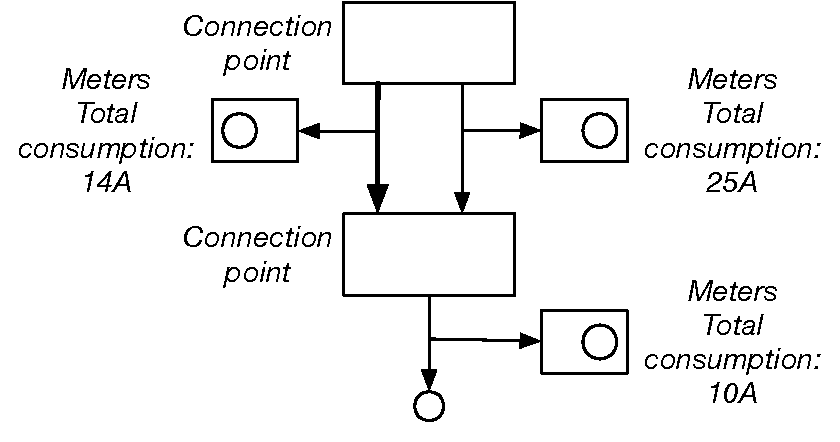
\includegraphics[width=.45\linewidth]{img/chapt-example/duc/Topology1-short}
		\label{fig:intro-schema-topology1}
	}
	\hfill
	\subfloat[Electricity flow 2] {
		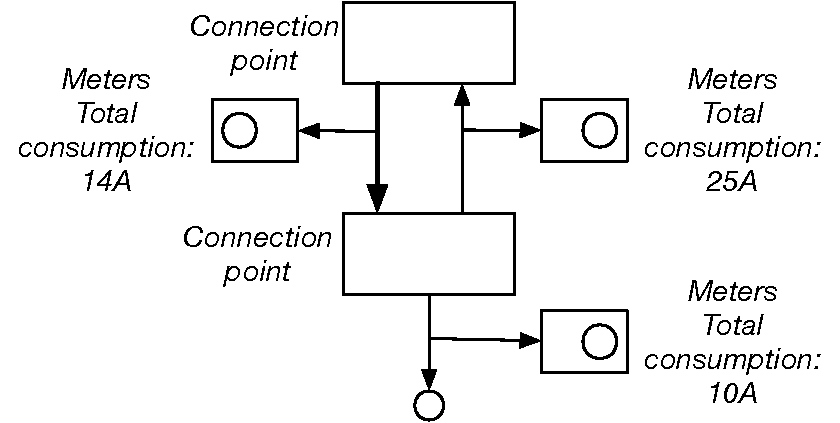
\includegraphics[width=.45\linewidth]{img/chapt-example/duc/Topology2-short}
		\label{fig:intro-schema-topology2}
	}
	\caption{Two different electric flows a same grid topology}
	\label{fig:intro-global}
\end{figure*}

%To exemplify how uncertainty may manifest in programs, we use a smart grid case study, built with Creos Luxembourg, our partner\footnote{Creos Luxembourg is the main grid operator in the country}. 
%More specifically, we focus on cable load estimation and the impacts of not taking uncertain into consideration. 
%We find that this case study is particularly appropriate to exemplify the concepts of uncertainty. 
%We highlight and discuss the limitations of existing approaches when handling such scenarios and show how and when our language is superior to these approaches.

%To exemplify how uncertainty may manifest in programs, we use a smart grid case study, built with a partner Creos Luxembourg\footnote{Creos Luxembourg is the main grid operator in the country. \url{https://www.creos-net.lu}}. 
%We focus on cable load estimation and the impacts of not taking uncertain into consideration. 
%We highlight and discuss the limitations of existing approaches when handling such scenarios.
%Plus, we show how and when our language is superior to these approaches.


%The National Institute of Standards and Technology (NIST) defines a smart grid as ``a planned nationwide network that uses information technology to deliver electricity efficiently, reliably, and securely"\footnote{\url{https://www.nist.gov/engineering-laboratory/smart-grid/smart-grid-beginners-guide}}.
%Conceptually, a smart grid is composed of different entities, like smart meters, cabinets (connection points of cables) and power substations.
%These entities are connected, forming a network, and able to exchange information using different technologies~\cite{DBLP:conf/smartgridcomm/0001FKTPTR14, DBLP:conf/sac/0001MFRKT16}.

%The network is the connection linking the smart grid entities by means of physical cables. 
%Every cable has a maximum load depending on its diameter and the used material.
%Figure~\ref{fig:intro-schema-physical} depicts an example of such a network. 
%This network is composed of one substation, one cabinet, and an arbitrary number of smart meters.
%Every cable has two fuses (to connect or disconnect the cable), one at each endpoint.
%By opening or closing fuses, one can influence the electricity flow through the network.
%Figure~\ref{fig:intro-schema-topology1} and~\ref{fig:intro-schema-topology2} show two possible electricity flows over the same physical network, illustrated in Figure~\ref{fig:intro-schema-physical}. 
%We depict closed fuses in black and the direction of the electricity flow using black arrows.

%Smart meters continuously measure electricity consumption and periodically report it to a central data centre.
%Based on this information, together with the grid topology, the electric load of cables can be computed.
%For example, the load on cable endpoint $i_1$ is equal to $\frac{iL_1 + iL_2 + iL_3}{2}$ in the first configuration and to $iL_1 + iL_2 + iL_3$ in the second one.
%With just one difference in one fuse state, there is a factor 2 of the load on $i_1$ between the two situations.
%If the reader wants to go more into the details of the calculation made, we invite him or her to read~\cite{DBLP:conf/sac/0001MFRKT16}.


Conceptually, a smart grid is a graph where the nodes represent the different entities (like meters, connection points of cables) and the edges represent physical cables.
Every cable has two fuses (to connect or disconnect the cable), one at each endpoint.
By opening or closing fuses, one can influence the electricity flow through the network.
Based on this flow and the electricity consumption, the grid manager can estimate the load in every cable.
This computation is detailed in~\cite{DBLP:conf/sac/0001MFRKT16}.

The flow has a big impact on the load cables.
In \autoref{fig:intro-global}, we depict two different flows for the same grid topology.
In both cases, the measured electric consumption are equal.
However, in \autoref{fig:intro-schema-topology1} the load on the left cable (thick line) equals $\frac{14 + 25 + 10}{2} = 24.5$ whereas it equals $14+25+10=49$ in \autoref{fig:intro-schema-topology2}.